\chapter{Régime transitoire des circuits linéaires}

\minitoc

\section{Généralités}

\subsection{Régime transitoire et régime permanent}

Par définition, le régime permanent est le régime où les grandeurs électriques ont des valeurs qui sont imposées par l'excitation (\ie le générateur).

Pour passer d'un régime permanent à un autre régime permanent, il faut temporairement passer par un régime transitoire.

Du point de vue mathématique, les grandeurs électriques sont solutions d'équations différentielles. Si \(y\) est une grandeur électrique alors \(y\paren{t}=y_P\paren{t}+y_G\paren{t}\) où \(y_P\paren{t}\) est une solution particulière et \(y_G\paren{t}\) la solution générale de l'équation homogène. \(y_P\paren{t}\) caractérise le régime permanent imposé par le générateur et \(y_G\paren{t}\) caractérise le régime transitoire du circuit.

On a \(y_G\paren{t}\xrightarrow[t\to\pinf]{}0\) donc à partir d'une certaine durée, le régime transitoire s'arrête et laisse place au régime permanent.

\subsection{Rappels sur les dipôles linéaires}

\subsubsection{Condensateurs}

\begin{circuit}
\draw (0,0) to[C,i>^=\(i\),v=\(u\),l=\(C\)] ++(3,0);
\end{circuit}

Un condensateur possède deux armatures métalliques en influence et porte la charge \(q\) :

\begin{tkz}
\draw[decoration={markings,mark=at position 0.5 with {\arrow{>}}},postaction={decorate}] (0,0) -- ++(2,0);
\draw (2,-2) -- (2,2) node[above left] {\(+q\)};
\draw (3,-2) -- (3,2) node[above right] {\(-q\)};
\draw (3,0) -- (5,0);
\foreach \x in {-1.8,-1.6,...,1.6,1.8} \node[right] at (2,\x) {\tiny+};
\foreach \x in {-1.8,-1.6,...,1.6,1.8} \node[left] at (3,\x) {\tiny-};
\node[above] at (1,0) {\(i\)};
\end{tkz}

On a : \[q=Cu\] avec \(C\) la capacité du condensateur (en farad : \(\unit{\farad}\)).

Comme \(i=\odv{q}{t}\), on a : \[i=C\odv{u}{t}.\]

On a la puissance reçue : \[P=ui=Cu\odv{u}{t}=\odv{}{t}\paren{\dfrac{1}{2}Cu^2}.\]

On a l'énergie stockée dans le condensateur : \[E=\dfrac{1}{2}Cu^2.\]

Comme \(P\not=\infty\), \(u\) est continue aux bornes du condensateur.

Condensateur réel : l'isolant entre les armatures n'est pas parfait donc il existe un courant de fuite à travers le condensateur.

Modèle du condensateur réel :

\begin{circuit}
\draw (0,0) -- ++(1,0);
\draw (1,1) -- (1,-1);
\draw (1,1) to[C,l=\(C\)] ++(2,0);
\draw (1,-1) to[R,l_=\(R\)] ++(2,0);
\draw (3,1) -- (3,-1);
\draw (3,0) -- (4,0);
\end{circuit}

avec \(R\approx\SI{e8}{\ohm}\).

Ordre de grandeur de la capacité : \(\unit{\micro\farad}\) à \(\unit{\nano\farad}\).

\subsubsection{Bobines}

\begin{circuit}
\draw (0,0) to[L,i>^=\(i\),v=\(u\),l=\(L\)] ++(3,0);
\end{circuit}

Ordre de grandeur de l'inductance : \(\unit{\milli\henry}\).

On a \[u=L\odv{i}{t}.\]

On a donc la puissance reçue \[P=ui=Li\odv{i}{t}=\odv{}{t}\paren{\dfrac{1}{2}Li^2}.\]

On a donc l'énergie emmagasinée dans la bobine : \[E=\dfrac{1}{2}Li^2.\]

De plus, on a \(P\not=\infty\) donc \(i\) est continue dans une bobine.

Bobine réelle : on fabrique une bobine en enroulant un fil autour d'un axe. Le fil étant résistif, le modèle de la bobine réelle est le suivant :

\begin{circuit}
\draw (0,0) to[L,l=\(L\),v=\(u\),i>^=\(i\)] ++(3,0) to [R,l=\(R\)] ++(3,0);
\end{circuit}

Avec \(R\) entre \(\SI{10}{\ohm}\) et \(\SI{100}{\ohm}\).

\section{Circuit RC série}

\subsection{Régime libre}

On considère le circuit suivant :

\begin{circuit}
\draw (0,0) to[cosw,i>^=\(i\),l=\(K\)] ++(3,0) to[R,l_=\(R\),v^=\(u_R\)] ++(0,-3) -- ++(-3,0) to[C,l_=\(C\),v^>=\(u_C\)] ++(0,3);
\end{circuit}

À l'instant \(t=0^-\), le condensateur est chargé sous une tension \(u_C\paren{t=0^-}=E\). À \(t=0\), on ferme \(K\).

D'après la loi des mailles, on a : \[u_C-u_R=0.\]

D'après les caractéristiques des dipôles, on a : \[i=-C\odv{u_C}{t}\quad\text{et}\quad u_R=Ri.\]

D'où \(u_C-Ri=0\) et donc : \[u_C+RC\odv{u_C}{t}=0.\]

On a une équation différentielle linéaire d'ordre 1 à coefficients constants et homogène. On la réécrit comme suit : \[\odv{u_C}{t}+\dfrac{1}{RC}u_C=0.\]

On pose \[\tau=RC\] la constante de temps du circuit RC.

On a : \[\begin{aligned}
\odv{u_C}{t}+\dfrac{1}{\tau}u_C&=0 \\
\odv{u_C}{t}&=-\dfrac{1}{\tau}u_C \\
\int\dfrac{\odif{u_C}}{u_C}&=\int-\dfrac{\odif{t}}{\tau} \\
\ln u_C&=-\dfrac{t}{\tau}+\mu \\
u_C\paren{t}&=\e{\mu}\e{-\frac{t}{\tau}}.
\end{aligned}\]

On pose \(\lambda=\e{\mu}\) et on obtient : \[u_C\paren{t}=\lambda\e{-\frac{t}{\tau}}.\]

On détermine \(\lambda\) avec la condition initiale : \(u_C\paren{t=0^-}=E\).

Comme la tension aux bornes d'un condensateur est continue, on a : \[u_C\paren{t=0^-}=u_C\paren{t=0^+}=E.\]

Donc \(\lambda\e{0}=E\) donc \[\lambda=E.\]

Finalement, on a : \[u_C\paren{t}=E\e{-\frac{t}{\tau}}.\]

De plus, on a : \[\begin{aligned}
i\paren{t}&=-C\odv{u_C}{t} \\
&=\dfrac{1}{\tau}EC\e{-\frac{t}{\tau}} \\
&=\dfrac{EC}{RC}\e{-\frac{t}{\tau}} \\
&=\dfrac{E}{R}\e{-\frac{t}{\tau}}
\end{aligned}\]

On obtient les graphes suivants (RP et RT signifiant respectivement \guillemets{régime permanent} et \guillemets{régime transitoire}) :

\begin{center}
\begin{tikzpicture}
\begin{axis}[axis lines=middle,
xlabel={\(t\)},
ylabel={\(u_C\)},
xmin=-4,xmax=16,
ymin=0,ymax=7,
xtick={3},
xticklabels={\(\tau\)},
ytick={1.84,5},
yticklabels={\(\dfrac{1}{\e{}}E\),\(E\)},
clip=false]
\addplot[domain=0:16,samples=1000,smooth,thick,blue] {5*exp(-x/3)};
\addplot[domain=-4:0,samples=1000,smooth,thick,blue] {5};
\draw (0,5) -- (3,0);
\draw[dashed] (3,0) -- (3,1.84) -- (0,1.84);
\draw[dashed,->] (-4,6) -- (0,6);
\draw[<->] (0,6) -- (12,6);
\draw[<-] (12,6) -- (16,6);
\node[above] at (-2,6) {RP};
\node[above] at (6,6) {RT};
\node[above] at (14,6) {RP};
\end{axis}
\end{tikzpicture}
\hskip10pt
\begin{tikzpicture}
\begin{axis}[axis lines=middle,
xlabel={\(t\)},
ylabel={\(i\)},
xmin=-4,xmax=16,
ymin=0,ymax=7,
xtick={0},
xticklabels={\(0\)},
ytick={5},
yticklabels={\(\dfrac{E}{R}\)},
clip=false]
\addplot[domain=0:16,samples=1000,smooth,thick,blue] {5*exp(-x/3)};
\draw[{}-{Arc Barb [length=0.1cm]},thick,blue] (-4,0) -- (0,0);
\node[below] at (0,0) {\(0\)};
\end{axis}
\end{tikzpicture}
\end{center}

\(\tau\) est appelé constante de temps du circuit, temps caractéristique ou temps de relaxation du circuit.

Temps de réponse à 5\% : on cherche \(t_\text{5\%}\) tel que \(u_C\paren{t_\text{5\%}}\) diffère de 5\% de sa valeur finale : \[u_C\paren{t_\text{5\%}}=\num{0.05}E=E\e{-\frac{t_\text{5\%}}{\tau}}.\]

On a : \[\begin{aligned}
\num{0.05}&=\e{-\frac{t_\text{5\%}}{\tau}} \\
\ln\num{0.05}&=-\dfrac{t_\text{5\%}}{\tau} \\
t_\text{5\%}&=\tau\ln20 \\
&=3\tau.
\end{aligned}\]

On trouve de même : \[t_\text{10\%}=5\tau.\]

Finalement, on obtient que le régime transitoire dure de \(3\tau\) à \(5\tau\).

\subsection{Réponse à un échelon de tension}

On considère le circuit suivant :

\begin{circuit}
\draw (0,0) to[cosw,i>^=\(i\),l=\(K\)] ++(3,0) to[C,l_=\(C\),v^=\(u_C\)] ++(3,0) to[R,l_=\(R\),v^=\(u_R\)] ++(0,-3) -- ++(-6,0) to[vsource,v^=\(E\)] ++(0,3);
\end{circuit}

À \(t=0^-\), le condensateur est de charge \(u_C\paren{t=0^-}=0\). À \(t=0\), on ferme \(K\).

D'après la loi des mailles, on a : \[u_R+u_C-E=0.\]

D'après les caractéristiques des dipôles, on a : \[u_R=Ri\quad\text{et}\quad i=C\odv{u_C}{t}.\]

D'où l'équation différentielle : \[RC\odv{u_C}{t}+u_C-E=0.\]

On pose \(\tau=RC\) et on obtient : \[\odv{u_C}{t}+\dfrac{1}{\tau}u_C=\dfrac{E}{\tau}.\]

Donc \[u_C\paren{t}=u_P+u_H\paren{t}\] où \begin{description}
\item \(u_P\) est une solution particulière de l'équation différentielle
\item \(u_H\) est la solution de l'équation homogène. \\
\end{description}

On a l'équation homogène \(\odv{u_C}{t}+\dfrac{1}{\tau}u_C=0\) donc \[u_H\paren{t}=\lambda\e{-\frac{t}{\tau}}.\]

\attention On ne détermine pas \(\lambda\) immédiatement car \(u_H\) n'est pas solution de l'équation complète !

De plus, on a \[u_P\paren{t}=\cte\] car \(\dfrac{E}{\tau}\) est une constante.

On a : \[\begin{aligned}
\odv{u_P}{t}+\dfrac{1}{\tau}u_P&=\dfrac{E}{\tau} \\
\dfrac{1}{\tau}u_P&=\dfrac{E}{\tau} \\
u_P&=E.
\end{aligned}\]

Finalement, on a : \[u_C\paren{t}=E+\lambda\e{-\frac{t}{\tau}}.\]

On détermine \(\lambda\) avec la condition initiale : \(u_C\paren{t=0^-}=0\).

Comme la tension aux bornes d'un condensateur est continue, on a : \[u_C\paren{t=0^-}=u_C\paren{t=0^+}=0.\]

Donc \(E+\lambda\e{0}=0\) donc \[\lambda=-E.\]

Finalement, on a : \[u_C\paren{t}=E-E\e{-\frac{t}{\tau}}=E\paren{1-\e{-\frac{t}{\tau}}}.\]

De plus, on a : \[i\paren{t}=\dfrac{E}{R}\e{-\frac{t}{\tau}}.\]

On obtient les graphes suivants :

\begin{center}
\begin{tikzpicture}
\begin{axis}[axis lines=middle,
xlabel={\(t\)},
ylabel={\(u_C\)},
xmin=-4,xmax=16,
ymin=0,ymax=7,
xtick={3},
xticklabels={\(\tau\)},
ytick={3.16,5},
yticklabels={\(1-\dfrac{1}{\e{}}E\),\(E\)},
clip=false]
\addplot[domain=0:16,samples=1000,smooth,thick,blue] {5*(1-exp(-x/3))};
\addplot[domain=-4:0,samples=1000,smooth,thick,blue] {0};
\draw[dashed] (0,5) -- (16,5);
\draw (0,0) -- (3,5);
\draw[dashed] (3,0) -- (3,5);
\draw[dashed] (3,3.16) -- (0,3.16);
\draw[dashed,->] (-4,6) -- (0,6);
\draw[<->] (0,6) -- (12,6);
\draw[<-] (12,6) -- (16,6);
\node[above] at (-2,6) {RP};
\node[above] at (6,6) {RT};
\node[above] at (14,6) {RP};
\node[below] at (0,0) {\(0\)};
\end{axis}
\end{tikzpicture}
\hskip10pt
\begin{tikzpicture}
\begin{axis}[axis lines=middle,
xlabel={\(t\)},
ylabel={\(i\)},
xmin=-4,xmax=16,
ymin=0,ymax=7,
xtick={0},
xticklabels={\(0\)},
ytick={5},
yticklabels={\(\dfrac{E}{R}\)},
clip=false]
\addplot[domain=0:16,samples=1000,smooth,thick,blue] {5*exp(-x/3)};
\draw[{}-{Arc Barb [length=0.1cm]},thick,blue] (-4,0) -- (0,0);
\node[below] at (0,0) {\(0\)};
\end{axis}
\end{tikzpicture}
\end{center}

\subsection{Aspect énergétique}

On considère le circuit suivant :

\begin{circuit}
\draw (0,0) to[cosw,i>^=\(i\),l=\(K\)] ++(3,0) to[C,l_=\(C\),v^=\(u_C\)] ++(3,0) to[R,l_=\(R\),v^=\(u_R\)] ++(0,-3) -- ++(-6,0) to[vsource,v^=\(E\)] ++(0,3);
\end{circuit}

On a : \[u_C\paren{t}=E\paren{1-\e{-\frac{t}{\tau}}}.\]

D'après la loi des mailles on a : \[\begin{WithArrows}
u_C+Ri&=E \Arrow{\(\times i\)} \\
iu_C+Ri^2&=Ei \\
Cu_C\odv{u_C}{t}+Ri^2&=Ei.
\end{WithArrows}\] où \begin{description}
\item \(Ei\) : puissance fournie par le générateur
\item \(Ri^2\) : puissance reçue par la résistance
\item \(Cu_C\odv{u_C}{t}=\odv{}{t}\paren{\dfrac{1}{2}Cu_C^2}\) : puissance reçue par le condensateur. \\
\end{description}

On en déduit \(E=\dfrac{1}{2}Cu_C^2\) l'énergie stockée par le condensateur.

Pour passer de la puissance à l'énergie, on intègre : \[\int_0^{\pinf} Ei\odif{t}=\int_0^{\pinf} Ri^2\odif{t}+\int_0^{\pinf}\odv{}{t}\paren{\dfrac{1}{2}Cu_C^2}\odif{t}.\]

On a : \[\int_0^{\pinf}Ei\odif{t}=\int_{q\paren{t=0}}^{q\paren{t=\pinf}}E\odif{q}\] car \(i=\odv{q}{t}\) où \(q\) est la charge portée par le condensateur.

Or on a : \[q\paren{t=0}=Cu_C\paren{t=0}=CE\paren{1-\e{0}}=0\quad\text{et}\quad q\paren{t=\pinf}=CE.\]

Donc on a : \[\int_0^{\pinf}Ei\odif{t}=\int_0^{CE}E\odif{q}=CE^2.\]

Donc \(CE^2\) est l'énergie fournie par le générateur entre \(t=0\) et \(t=\pinf\) (\ie au cours de la charge du circuit).

De plus, on a : \[\int_0^{\pinf}\odv{}{t}\paren{\dfrac{1}{2}Cu_C^2}\odif{t}=\int_0^{\frac{1}{2}CE^2}\odif{\paren{\dfrac{1}{2}Cu_C^2}}=\dfrac{1}{2}CE^2.\]

Finalement, on a : \[\int_0^{\pinf}Ri^2\odif{t}=\int_0^{\pinf}Ei\odif{t}-\int_0^{\pinf}\odv{}{t}\paren{\dfrac{1}{2}Cu_C^2}\odif{t}=CE^2-\dfrac{1}{2}CE^2=\dfrac{1}{2}CE^2.\]

D'où le bilan d'énergie entre \(t=0\) et \(t=\pinf\) : \begin{description}
\item Énergie fournie par le générateur : \(CE^2\)
\item Énergie reçue par le condensateur : \(\dfrac{1}{2}CE^2\)
\item Énergie reçue par la résistance (dissipée par effet Joule) : \(\dfrac{1}{2}CE^2\). \\
\end{description}

On définit le rendement : \[\eta=\dfrac{\text{énergie utile}}{\text{énergie fournie}}.\]

Ici, on a : \[\eta=\dfrac{\frac{1}{2}CE^2}{CE^2}=\dfrac{1}{2}=50\%.\]

\note{À FINIR}